

\newcount\draft\draft=1 % set to 0 for submission or publication
\newcount\cameraready\cameraready=1


\documentclass[conference]{IEEEtran}

\usepackage{graphicx}
\DeclareGraphicsExtensions{.pdf,.jpg,.png}
\graphicspath{{./figs/} {./plots/}}

\usepackage{balance}
\usepackage{comment}
\usepackage{xspace}
\usepackage{xxx}
\usepackage[export]{adjustbox}
\usepackage{wrapfig}
\usepackage{multicol}
\usepackage{float}
\usepackage{subfigure}
\newcommand{\sys}{Safewalk\xspace}
\newcommand{\utodo}[2]{ {\textcolor{red} {#1}}: {\textcolor{red} {#2}}}
\author{
  \IEEEauthorblockN{
   Iljoo Baek, Mengwen He and Emily Ruppel
  }
 \IEEEauthorblockA{
   Carnegie Mellon University
  }
 \IEEEauthorblockA{
   {ibaek,mengwenhe,eruppel}@andrew.cmu.edu
  }
}
\title{Gait Monitoring using Wireless Sensors\\
        \vspace{4mm}
        \large{Final Report 18-748}\\
        \large{Spring 2017}}

\begin{document}

\maketitle
\thispagestyle{plain}
\pagestyle{plain}

%Only including an abstract since it looks like the submission site wants one... 
\begin{abstract}
In this project we demonstrate \sys, a gait monitoring system comprised of Firefly wireless
sensor motes that relay data from inertial measurement units mounted on a subject's body
to a central server. Using the acceleration and orientation information reported at six
different points along a subject's legs and feet, we were able to visualize the subject's
movements in real time and capture the relevant motion data to be used for future
analysis. Our system also provides a low-processing solution for fall detection through
thresholding analysis of the orientation measurements reported by a subset of the sensor
nodes in the system. After testing our system on three different subjects, we believe it
represents a proof of concept of low cost gait monitoring systems that will improve the
quality of patient care in a multitude of settings. 
\end{abstract}

\section{Introduction}
  \label{sec:intro}
  Gait patterns, the measurable characteristics of an individual’s walking movement, can
provide insight into a variety of components of an individual’s health status. Certain
gait pathologies may be associated with specific medical conditions. Sudden changes in the
way an individual walks can be indicative of the occurrence of an undetected but
deleterious medical event, i.e. undetected stroke. A shift in gait pattern over time may
come about as the result of muscular or neural decline that could increase the probability
of a dangerous event, such as a fall, in the future. However, diagnosing conditions or
predicting an increased fall risk from gait patterns requires the attention of a trained
medical professional, which limits the settings in which gait analysis can be used.
    
Wireless Body Area Networks have been proposed as a promising solution for capturing
useful health status indicators without inconveniencing a patient~\cite{msban,wban}. The
additional data enables a new field of computer-assisted physical therapy that allows
therapists to deliver more targeted care to their patients. Advanced treatment centers for
patients with unique cases, such as the Walter Reed Center for Performance and Clinical
Research (CPCR) amputee clinic, use extensive computer modeling to aid in patient
rehabilitation~\cite{cpcr}.  An apparent barrier to the widespread adoption of computer
assisted therapy is the cost of the motional analysis systems. For instance, the CPCR uses
23 infrared cameras to track the movement of reflective markers attached to a patient's
body and six force plates in the floor to fully capture a patient's movement. Though the
movement data can be captured and used at a later time, the gait analysis is still limited
to a clinical setting. 
  
\sys's goal was to expand the usefulness of gait analysis beyond a professional’s
office to an individual’s day-to-day environment. We accomplished our goal by
demonstrating a proof-of-concept gait monitoring system that relies on wireless motes
instrumented with Inertial Measurement Units (IMUs) to capture relevant data and relay
them to a powerful backend machine for offline and real time processing. Our system
extracted a variety of components of the subject's gait pattern from linear and angular
acceleration data measured at specfic points along his or her legs. The subject's
movements were then visualized and features of the gait were plotted in real time. We also
demonstrate the practicality of real-time fall detection by using a simple thresholding
technique to indicate when a subject is no longer upright. Throughout the trials with our
prototype system we note that wireless sensor networks are particularly promising for
accomplishing gait detection because the small nodes and lack of constraining wires
minimizes the impact on the patient and allows for an honest gait assessment without the
residual impact of cumbersome measurement devices. 
\section{Related Work}
This project is based on prior work in gait analysis and wireless sensors networks used to
aid healthcare objectives. In this section we will describe how the prior work influenced
the design of our project 
\subsection{Gait Analysis}
Gait analysis using wearable sensors is a well-studied approach to characterizing gait
patters~\cite{gaits}. The goal of the gait analysis approaches is to analyze the various phases of
the human gait to identify abnormalities. A normal walking gait is comprised of eight
stages as shown in Figure~\ref{fig:phases}. 

\begin{figure}[h]
  \centering
  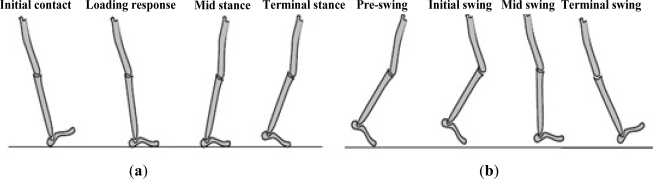
\includegraphics[width=0.9\columnwidth]{figs/phases}
  \caption{{\bf Phases of the stance (a) and swing (b) periods~\cite{gaits} }}
  \label{fig:phases}
\end{figure}

Since the first study using wearable sensors in 1973, researchers have captured the data
from these phases using a variety of transducers. Recently, multiple studies have used
IMUs attached to a subject’s thigh, calf, and foot to study gait kinematics. Gait
kinematics investigates the movement of segments of the lower limbs while walking or
running~\cite{run}. This is distinct from gait kinetics which analyzes the forces exerted on
different joints while walking. The difficulty with kinetic analysis is the hardware
required to capture accurate measurements. Previous studies have relied on specialized,
instrumented footwear that measures the forces acting on a patient’s foot. Gait
kinematics, on the other hand, has moved towards less intrusive measurement techniques.
For instance, ~\cite{walkers} used small wireless sensor nodes to report information about the gait
characteristics of test subjects. Graurock, et. al went one step further in targeting
patient convenience by building a "plug-and-play" system wherein each sensor node self
calculated its position on a patient's lower extremeties~\cite{pairing}.  

\subsection{IMU Data Processing}
A large amount of work has been performed in processing the acceleration and orientation
values reported by inertial measurement sensors to make use of the data. Specifically in
terms of gait analysis, the work comes from both the robotics and motion capture
communities. 
%Can we get a citation from the robotics community here too? 
For instance, Yost labs has characterized the different joint types of the
human body in terms of the necessary interpetation of data from IMUs mounted on adjacent
limbs~\cite{yost}. The complexity of the analysis ranges from the simple calculation to
determine the angle of a hinge joint to the vector transformations required to assess the
pitch, yaw and roll of multi-axis joints. Complementary work from the medical community
puts the raw measurements in context for clinicians by providing a point of comparison.
For instance, in ~\cite{pop} inertial sensor data was collected from a large population
of adults and translated into a database of typical gait parameter values that researchers
and healthcare professionals can use as a point of comparison. The study combines a
multitude of well characterized algorithms for assessing gait parameters using only two
IMUs, one on each of the subject's feet, and is able to build a model for normal gaits
in terms of parameters such as foot clearance and step cadence. 


\section{Technical Description}
Our system follows in the spirit of prior work using IMUs to measure gait parameters, and
work that uses wireless sensors to improve the quality of patient care. The system
architecture we employ to achieve our goal of measuring a subject's gait using wireless
sensors is shown in Figure~\ref{overview}. Note that it contains six Firefly slave devices
each with a Sparkfun Razor 9 DoF Razor IMU M0 board attached. The data are then
transmitted from the slave nodes to a master node which finally pushes the data to a
server. To implement our gait monitoring system we had to handle three major design
points- transmitting data from the IMUs, analyzing the IMU data, and building a useful
interface to the information. This section will describe the choices our team made with
regards to these three subsystems. 

\begin{figure}[h]
  \centering
  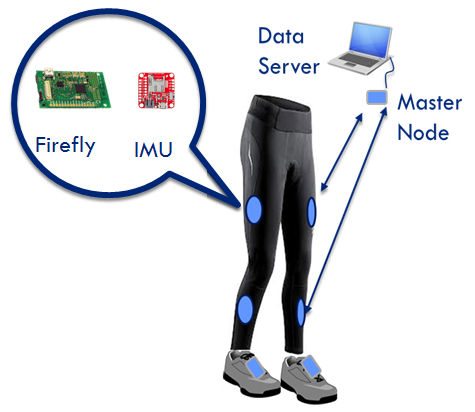
\includegraphics[width=0.75\columnwidth]{figs/sysarch}
  \caption{{\bf High level system design}}
  \label{fig:overview}
\end{figure}



\subsection{Device Communication}
Moving data from the IMU to the remote server can be separated into two distinct
transitions-- one from IMU to firefly slave device and another from the slave to the
master node. As shown in Figure~\ref{fig:ff}, the IMU board attaches directly to the
Firefly. The connection provides power from the Firefly batteries to the IMU and allows
for two way communication over one of the Firefly's auxiliary UART ports and the
configurable IMU communication ports. The majority of the data transported over the serial
connection is the IMU readings transported from the IMU board to the Firefly whenever the
IMU has data available. 

\begin{figure}[ht]
  \centering
  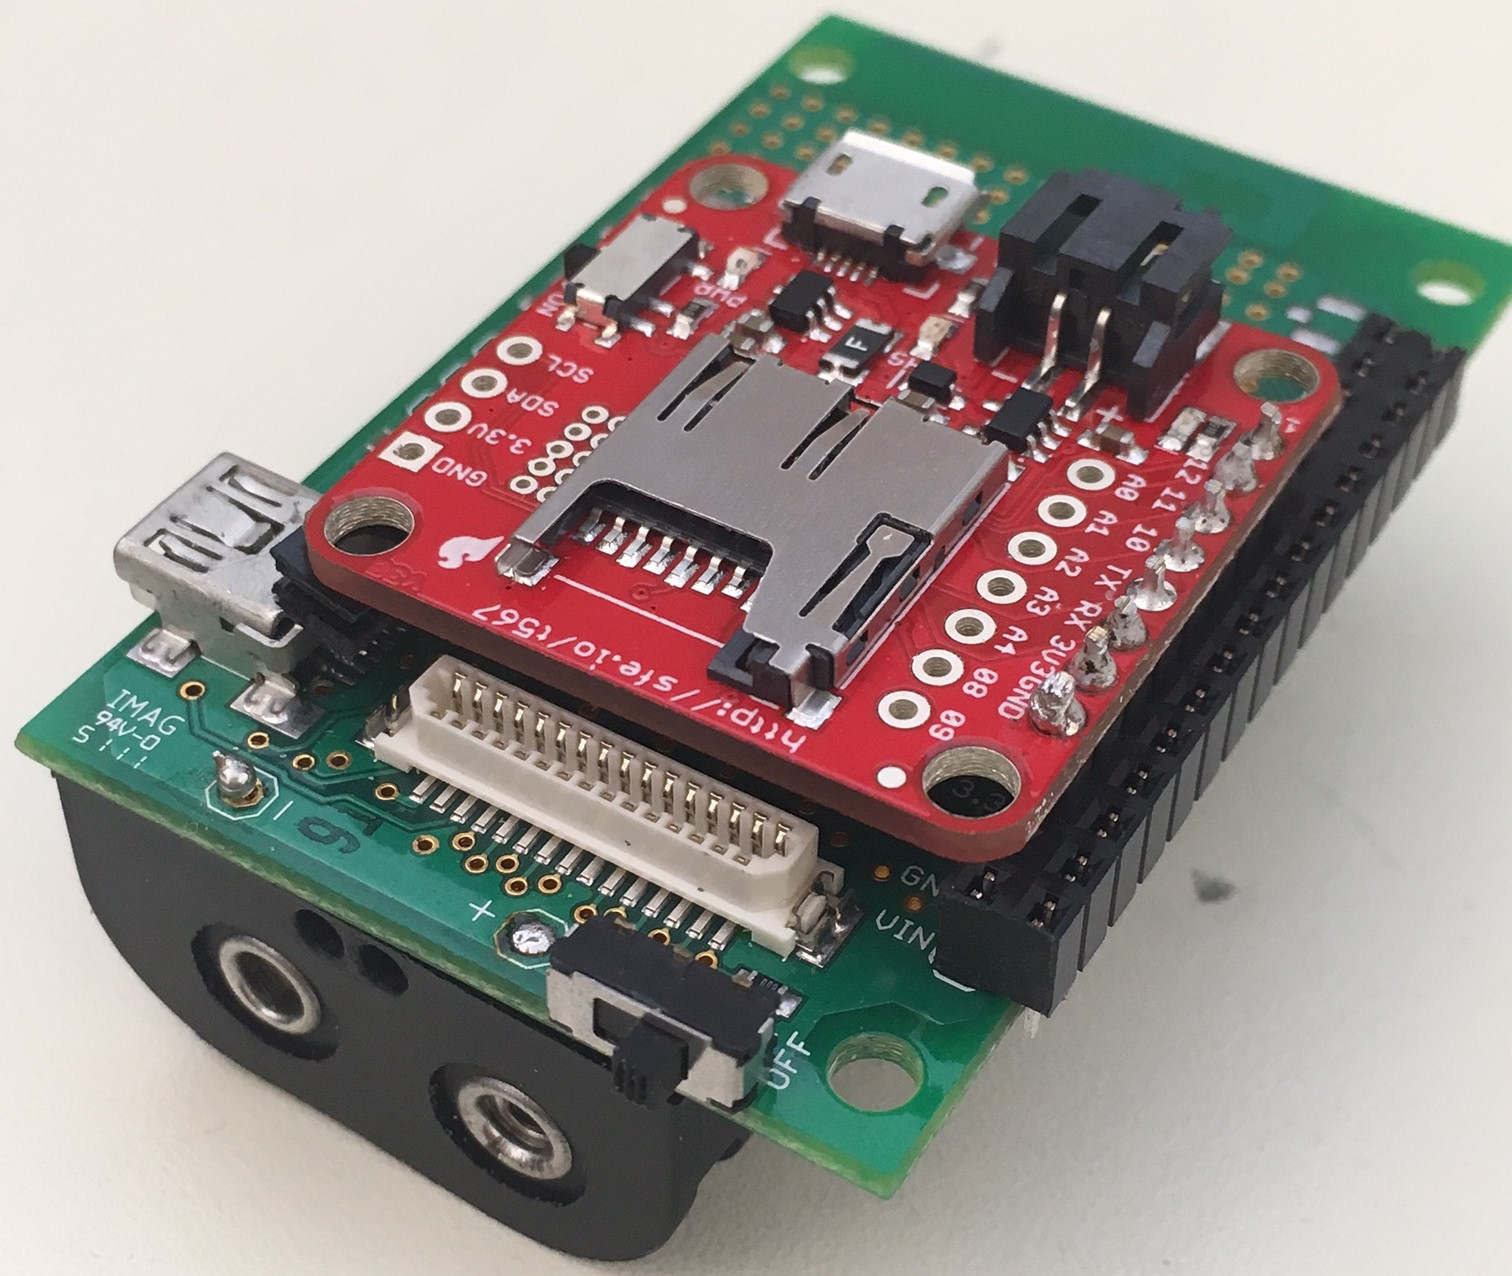
\includegraphics[width=0.6\columnwidth]{figs/cropped2}
  \caption{{\bf Firefly node with IMU board attached}}
  \label{fig:ff}
\end{figure}

  The format of the packet passed from IMU to Firefly is shown in
Figure ~\ref{fig:packet}. The data are encoded as ASCII characters to simplifiy debugging
as data move from IMU to firefly slave node to master and final output. While the ASCII
encoding greatly simplified debugging, it does mean that the packet size may change given
different accelerometer values.  Throughout the project, several unsuccessful attempts
were made to tightly control the data transmission by the IMU board, but the nature of the
UART protocol made timing discrepancies between the two devices difficult to overcome, and
was further complicated by the variable packet size. Instead, we settled on a four
character pattern to indicate the beginning of an IMU transmission followed by a single
special character to indicate the end. In contrast to the long packets transmitted from
the IMU board, the firefly needs only to issue commands to the IMU, so the protocol from
firefly to IMU is far simpler. If the IMU board receives a character from the Firefly, the
corresponding command is retrieved from a look-up table and carried out. A final feature
of the IMU-Firefly communication protocol is automatic reboot of the firefly. 

\begin{figure}[h]
  \centering
  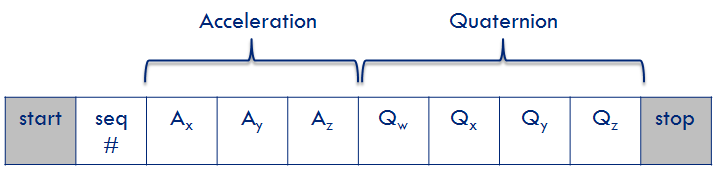
\includegraphics[width=0.8\columnwidth]{figs/packet}
  \caption{{\bf Packet Format from IMU to Firefly}}
  \label{fig:packet}
\end{figure}


Once packets are passed from the IMU to the Firefly slave device, the firefly transmits
the packet using the Point Coordination Function (PCF) TDMA protocol~\cite{pcf}. Each
slave device is statically assigned a time slot according to its preprogrammed MAC address
and only transmits during its assigned slot. The PCF TDMA protocol is designed for a
network with a star topology, where all slave nodes are within one hop of the master
device because all slave nodes must synchronize based on a message sent from the master at
the beginning of every TDMA cycle.  Despite its simplicity, this protocol met our design
goals of maximizing data throughput by preventing collisions without inucurring the time
overhead of carrier sense~\cite{CSMA}.  During its designated time slot, a slave node
transmits the packet passed to it from the IMU after stripping off the start and stop
bytes. An added advantage of the TDMA protocol is the implicit ID and time information
coupled with each transmission. Based on the time slot during which a packet is received,
the master node can automatically attach the ID of the node that transmitted the packet
before passing the entire packet to the server for processing. Further, the time
synchronization as a result of TDMA allows for the assumption that the measurements from
different IMUs received during a given TDMA cycle occurred at the same time. Therefore,
the server can afix a timestamp to data based on when it receives the data rather than
transmitting a timestamp from the slave node indicating the precise moment when the IMU
measurement was made. 

The protocol delivers a data rate of approximately 10 packets per second from each of
the slave nodes. This rate could be improved by decreasing the packet size, and more
tightly matching the TDMA slot length to the transmission time of a packet. In the current
configuration, the slot length is fixed at 10ms per node. Further exploration of the
transmit and receive task lengths on the slave nodes could also improve throughput.
Currently both the receive and transmit tasks operate on a period of 250ms. In the
transmit task, a slave device transmits as many times as possible given the tdma protocol
before switching to the receive task, but during the receive task the node will receive a
message with low probability because the master sends commands to the slaves infrequently.
Reducing the length of the receive period will thererfore reduce the slave node's idle
time with little impact on the system's performance. 

  The only command transmitted from the master to the slaves beyond the TDMA synchronization
is a "Recalibrate" command that signals the slave nodes to send messages to their IMUs to
perform static calibration. This command is sent only when a users pushes the auxiliary
button the master firefly at the beginning of a long period of system operation. While the
communication protocol is complicated by this single command, it is important that the
master node be able to issue a synchronous recalibration command to all of the nodes to
improve the accuracy of the following measurements. The recalibraton phase samples the
baseline static noise floor of each IMU, so the subject wearing the devices must be
stationary while the devices are undergoing recalibration. It is difficult for the subject
to remain stationary if each of the devices must be manually turned off and then on to initiate
recalibration. The master's recalibrate command circumvents the issue by causing all IMUs
to recalibrate instantaneously which greatly reduces the amount of time the patient must
remain still. 

\subsection{Gait Analysis}
Our work analyzing subject's gait parameters focused on stride length, swing time, and
knee extension. Each of these parameters required different analysis techniques that will
be described below.\\ 
{\bf Stride Length} To determine the stride length, we first assume that the lengths of each
segment of a subject's limbs are known. \utodo{Alex}{Describe how stride length was
calculated}
\\
{\bf Swing Time} Our analysis focuses on detecting the subject's step to in turn ascertain
when a subject's foot is on the ground, and when it is in motion. By making the assumption
that the acceleration of the foot is close to zero when it is on the ground, we were able
to detect the beginning and end of a subject's stride based strictly on acceleration data
from the x-y plane. Our implementation is a simplified version of the technique used
in~\cite{fancy}. Figure~\ref{fig:step-detect} shows the basic shape of accelerometer data
gathered from a subject's feet as he or she walks and the marked regions indicate the time
during which his/her foot is either on the ground or in the air. \\
\begin{figure}[h]
  \centering
  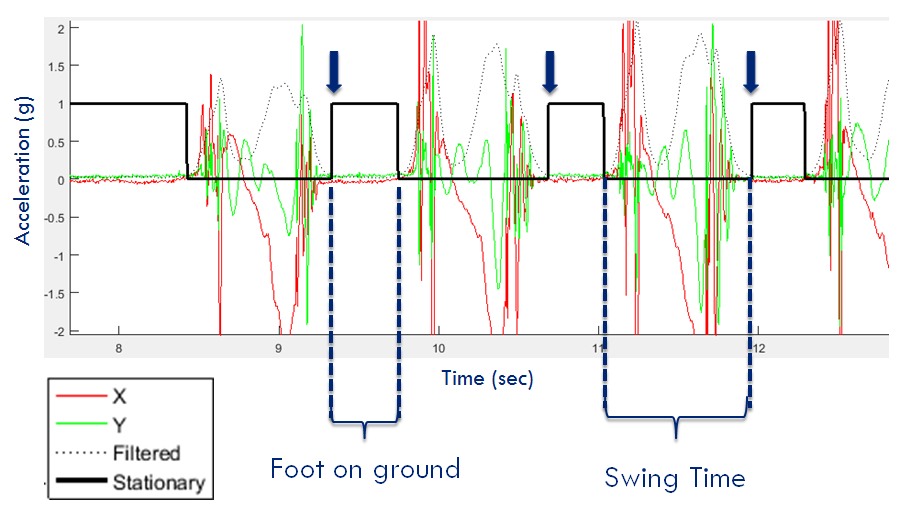
\includegraphics[width=0.8\columnwidth]{figs/swing}
  \caption{{\bf Step detection from accelerometer data}}
  \label{fig:step-detect}
\end{figure}
{\bf Knee Extension} A subject's knee extension was calculated using the hinge joint
techniques explained by Yost~\cite{yost}. The equations are \utodo{Iljoo}{Add the
equations you actually used for knee extension} Figure~\ref{fig:knees} shows the angles
that are reported by the final calculation. 

\begin{figure}[h]
  \centering
  \includegraphics[width=0.8\columnwidth]{figs/knees}
  \caption{{\bf Knee extension Calculation}}
  \label{fig:knees}
\end{figure}

\subsection{User Interface}
\utodo{Alex}{Add all the details about the user interface that I missed!!}
The user interface is aimed at a technical professional rather than a healthcare provider,
but it is built so that certain features are easy to access for non-technical personnel
and data storage for future processing is streamlined. Our design uses the popular Robot
Operating System (ROS) platform to control data flow into the system software from the
single stream of data coming from the master node. The control buttons for data from the
individual nodes are simple to access and can be used to change the system's
configuration. The interface also contains a slave node health status indicator that
reports whether or not the master node has successfully received data from a given slave
within a recent timeframe. Figure~\ref{fig:ROS} shows the configuration interface and the
health status indicator. In a healthcare environment, these tools would be used by
technical personnell to configure the system software before it is used by a healthcare
provider. 

\begin{figure}[h]
  \centering
  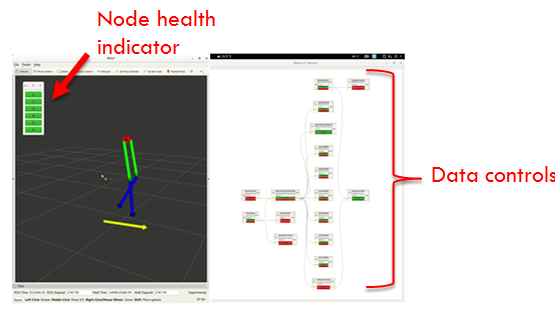
\includegraphics[width=\columnwidth]{figs/gui}
  \caption{{\bf ROS user interface}}
  \label{fig:gui}
\end{figure}
The user interface also provides a convenient video playback feature than can replay all
of the data visualizations produced in real time during active data capture as well as an
accompanying video of the subject. Finally, the data are logged automatically for future
use or offline analyses. 


\subsection{Enclosure} 
To ensure that the IMU remains in a fixed position on the body, and to protect the
connection between the Firefly and the IMU, we designed a 3D printed enclosure for the
slave nodes. Figure~\ref{fig:box} shows the enclosure with and without the specially designed
lid. The enclosure allows for easy access to all programming ports, power switches and
batteries without time consuming disassembly. Further, the design allows a strap to easily
pass through the upper and lower pieces of the enclosure so that the devices can be
comfortably affixed to subjects using velcro straps. During testing, we found that the
straps held the slave devices securely in place and they did not restrict the subject's
movements. 
%Except for that part where the ones on the thighs acted like tourniquets... but we won't
%talk about that... 
\begin{figure}[h]
  \centering
  \subfigure[]{
    \centering
    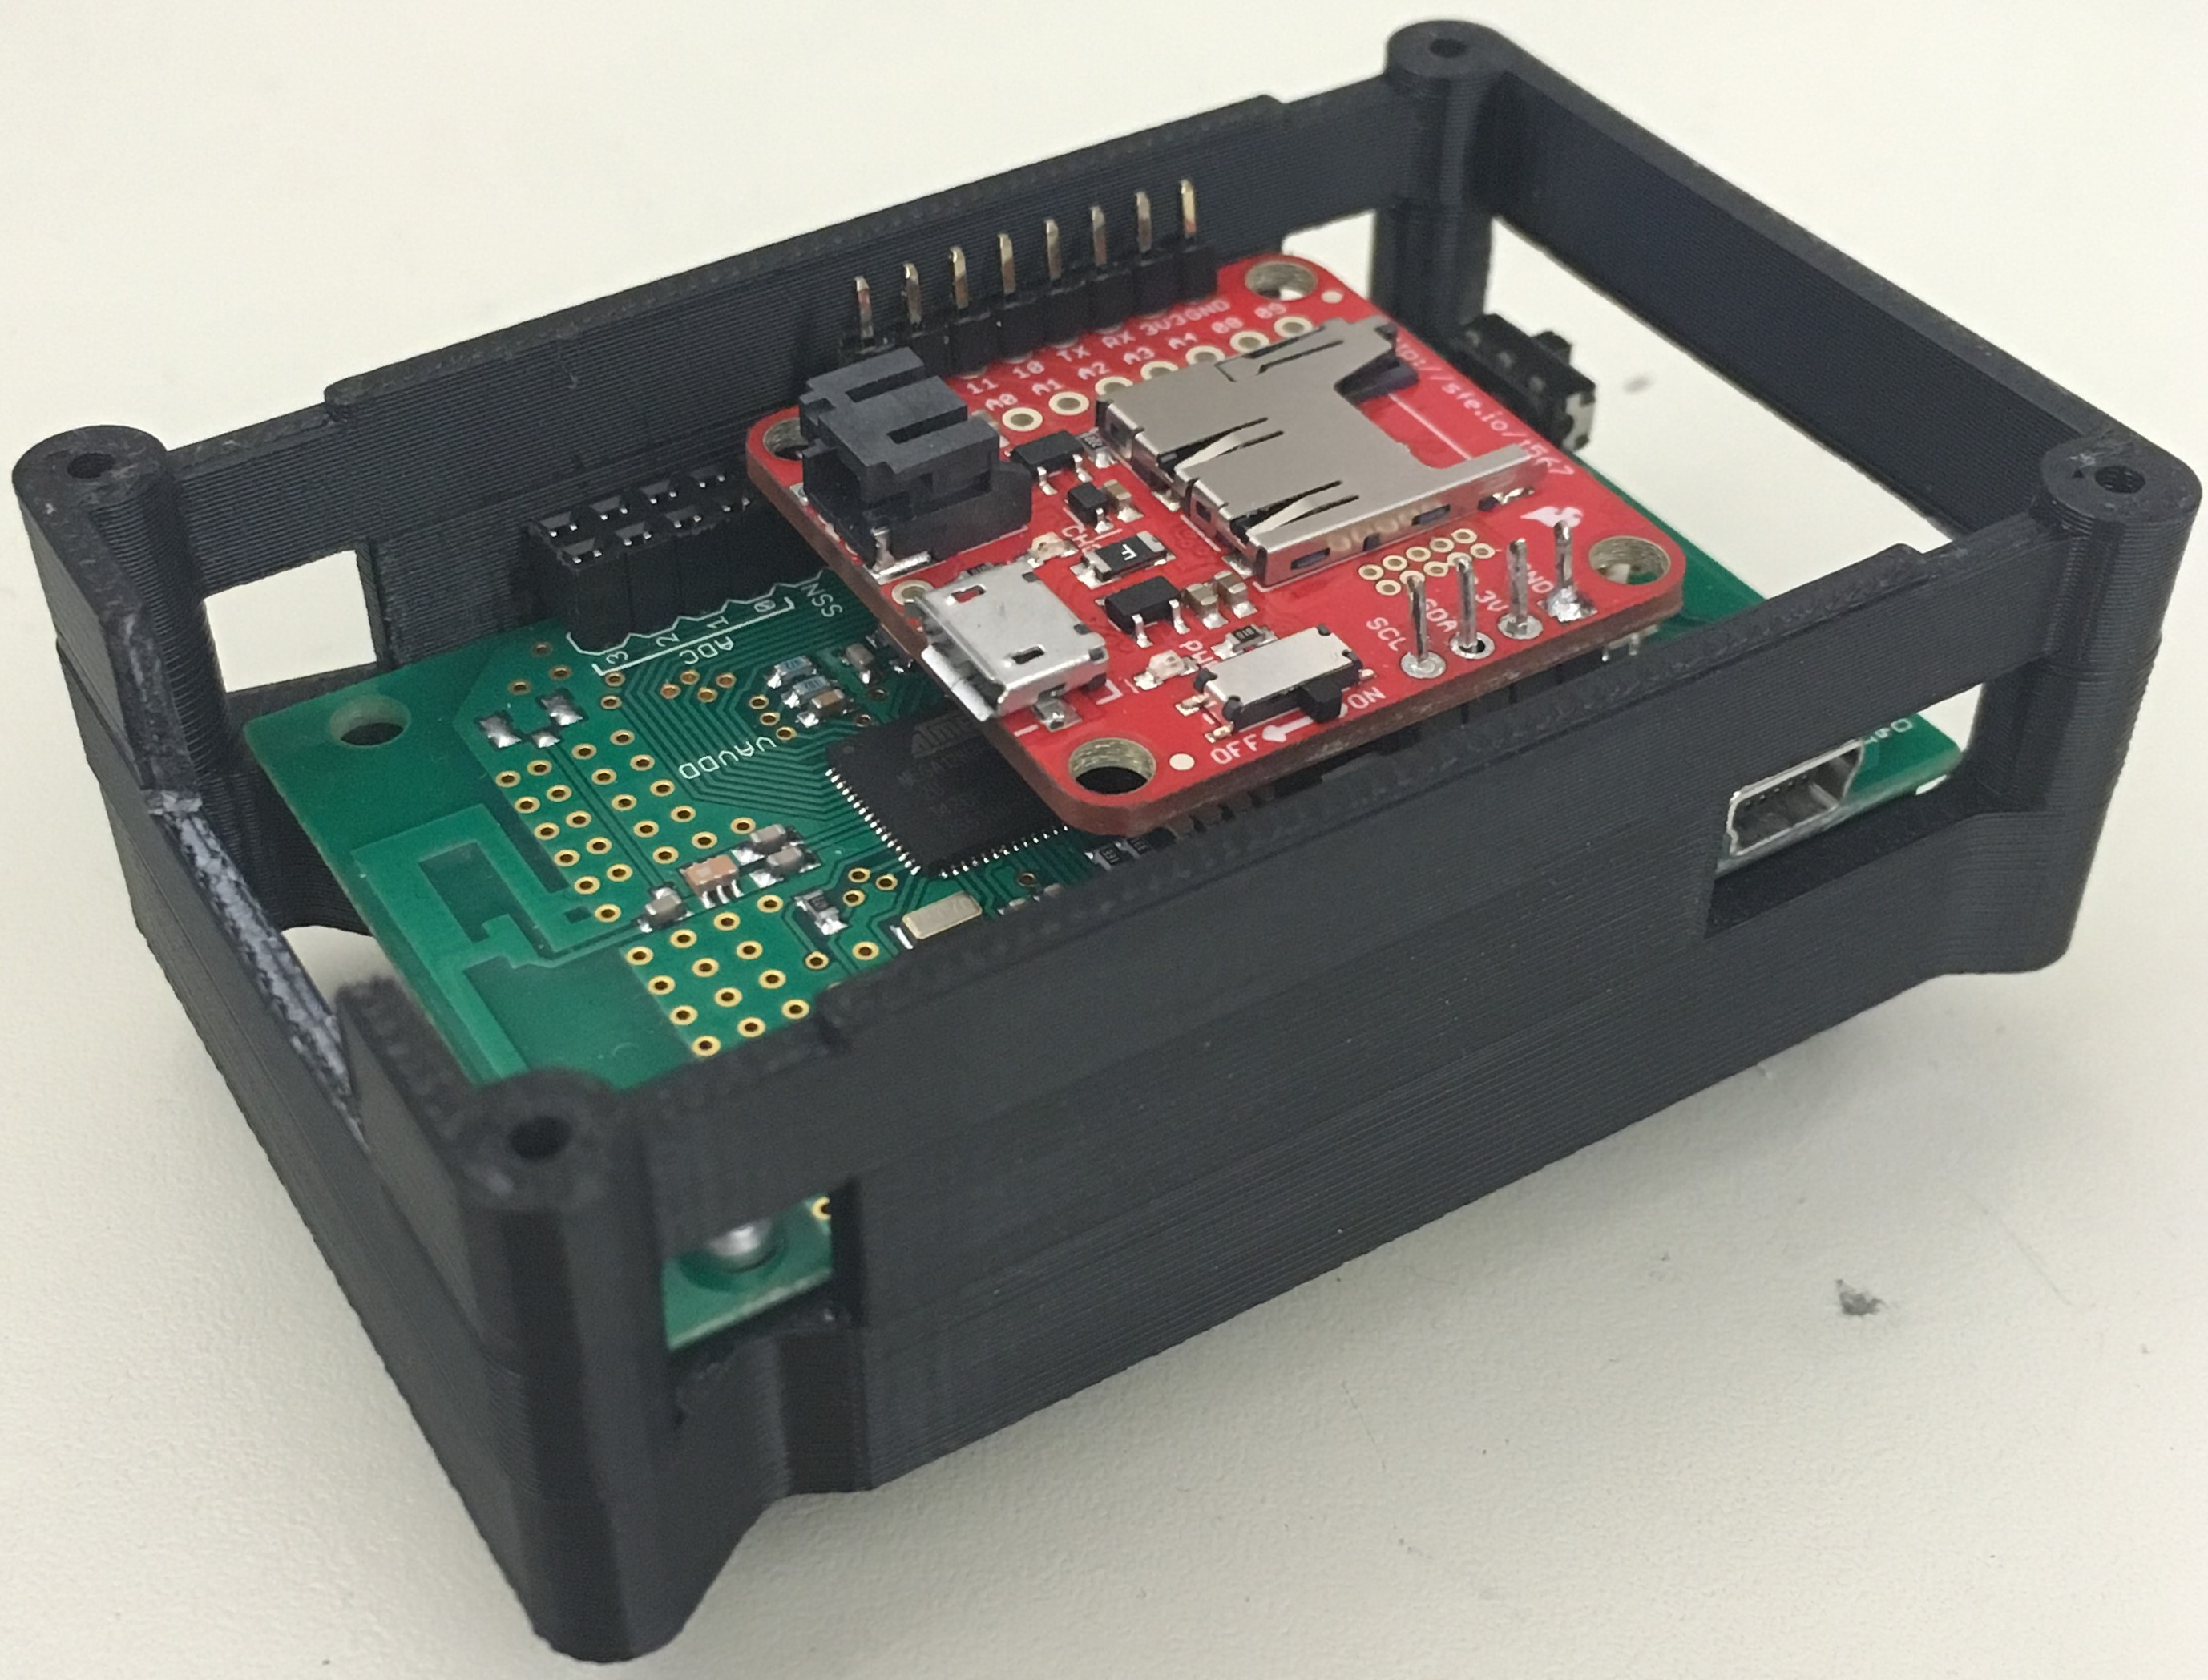
\includegraphics[width=.45\columnwidth]{figs/box}
    \label{fig:box2}
  }
  \subfigure[]{
    \centering
    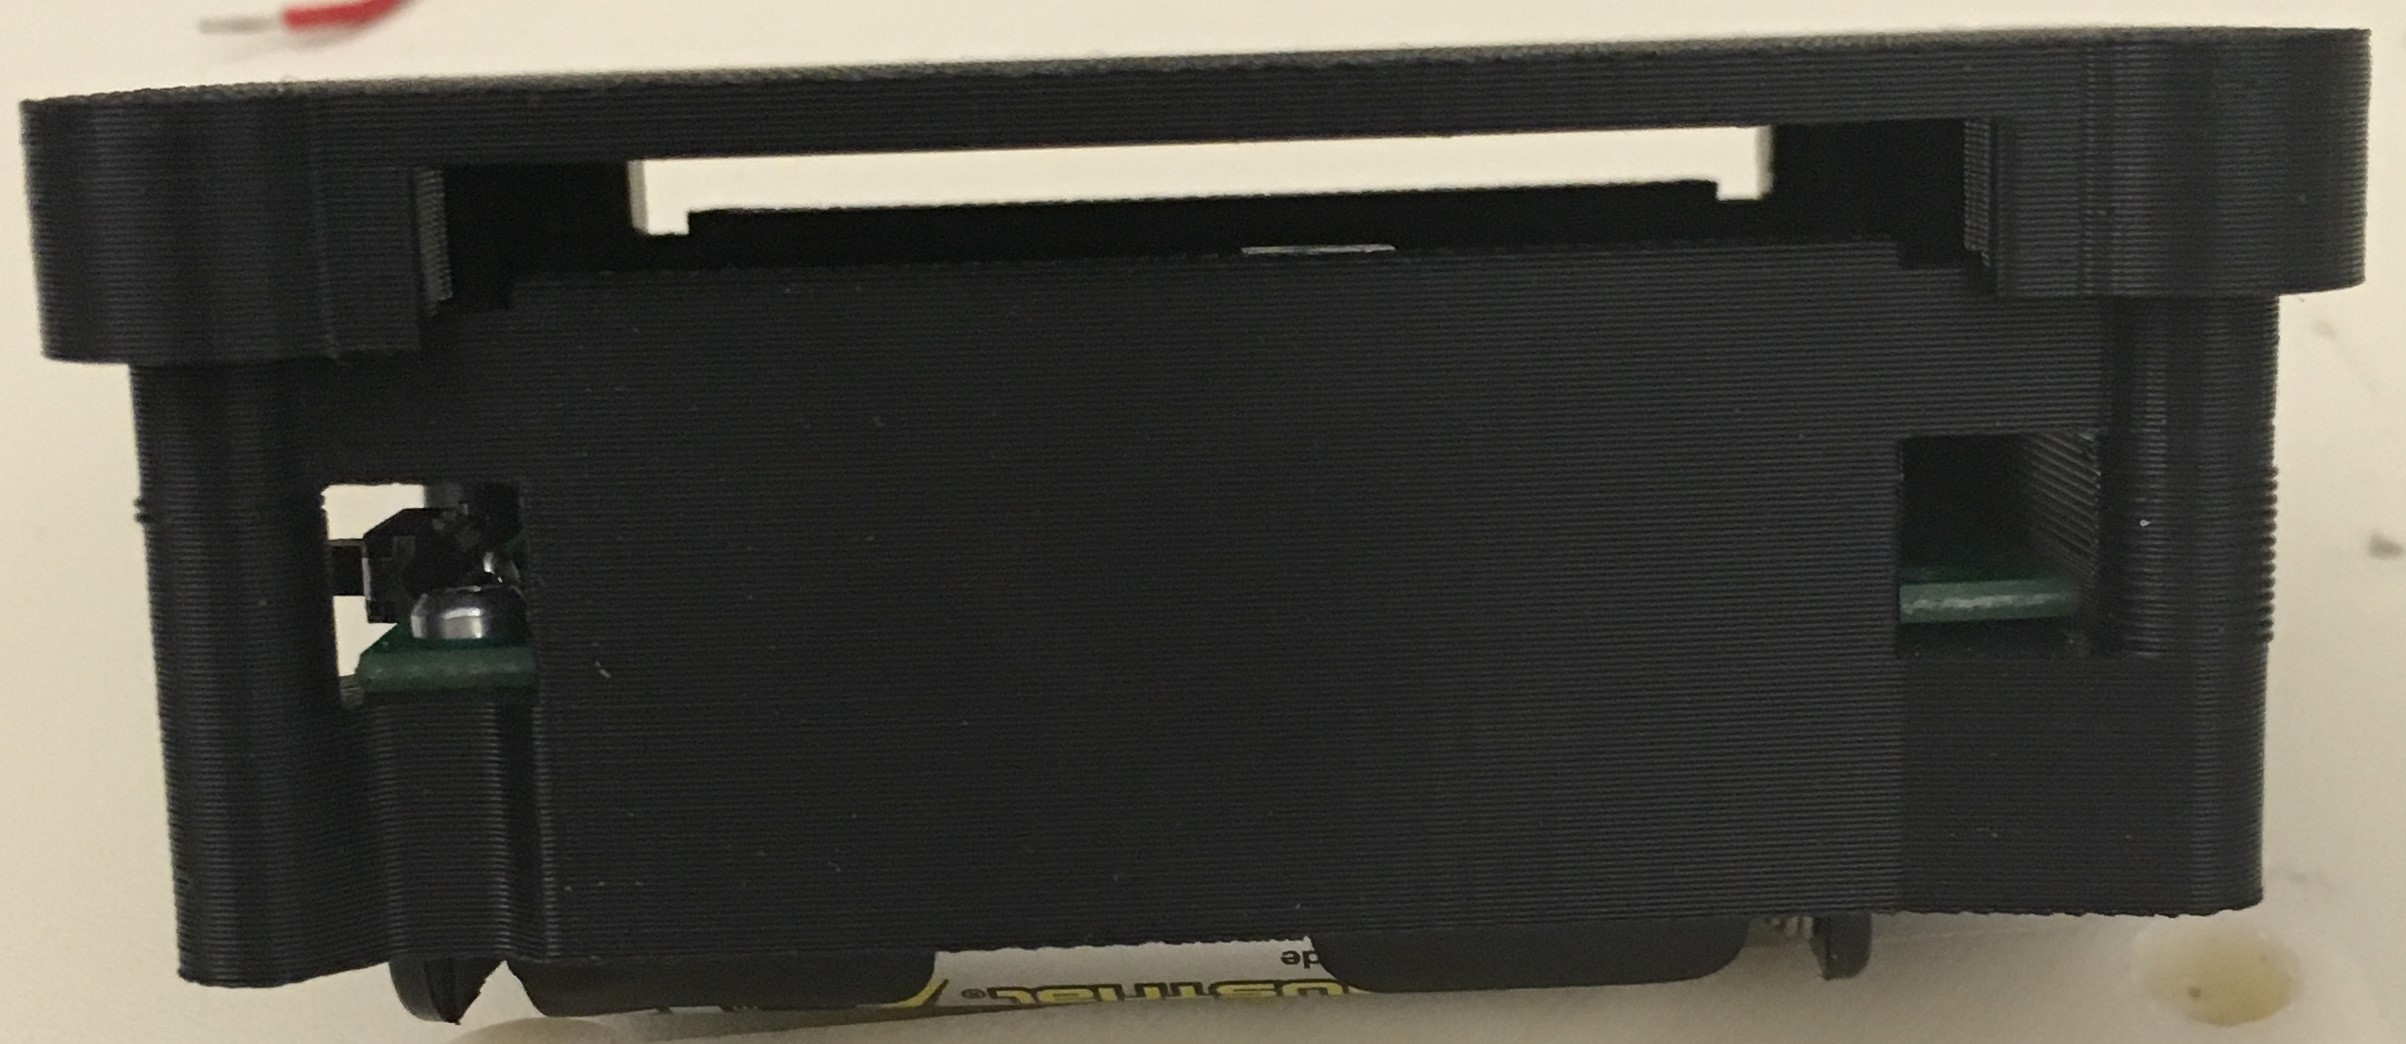
\includegraphics[width=.45\columnwidth]{figs/wLid}
    \label{fig:wLid}
  }
  \label{fig:box}
  \caption{{\bf Enclosure for sensor nodes}}
\end{figure}

\section{Results}
Our results are best demonstrated through a series of the screenshots acquired during
multiple demos. They capture the objective of our project and demonstrate the value of the
current prototype as well as the points where improvements could be made. 
\subsection{Visualization}
Our final data visualization included a simple avatar and representations of the
orientation of all six slave nodes. Figure~\ref{fig:vis} shows the final visualization layout.
Both elements of the visualization moved in real time as data passed in from the master.
For the orientations, each node's axes move independent of the other nodes, so the
movements provide the user with a sense of the raw noise included in the orientation
measurements. If any of the node's IMUs reports some kind of spurious, outlying data
point, the user will observe a sudden change in that IMU's axis representation. Future
work would filter out sudden changes to prevent this phenomena. 

\begin{figure}[h]
  \centering
  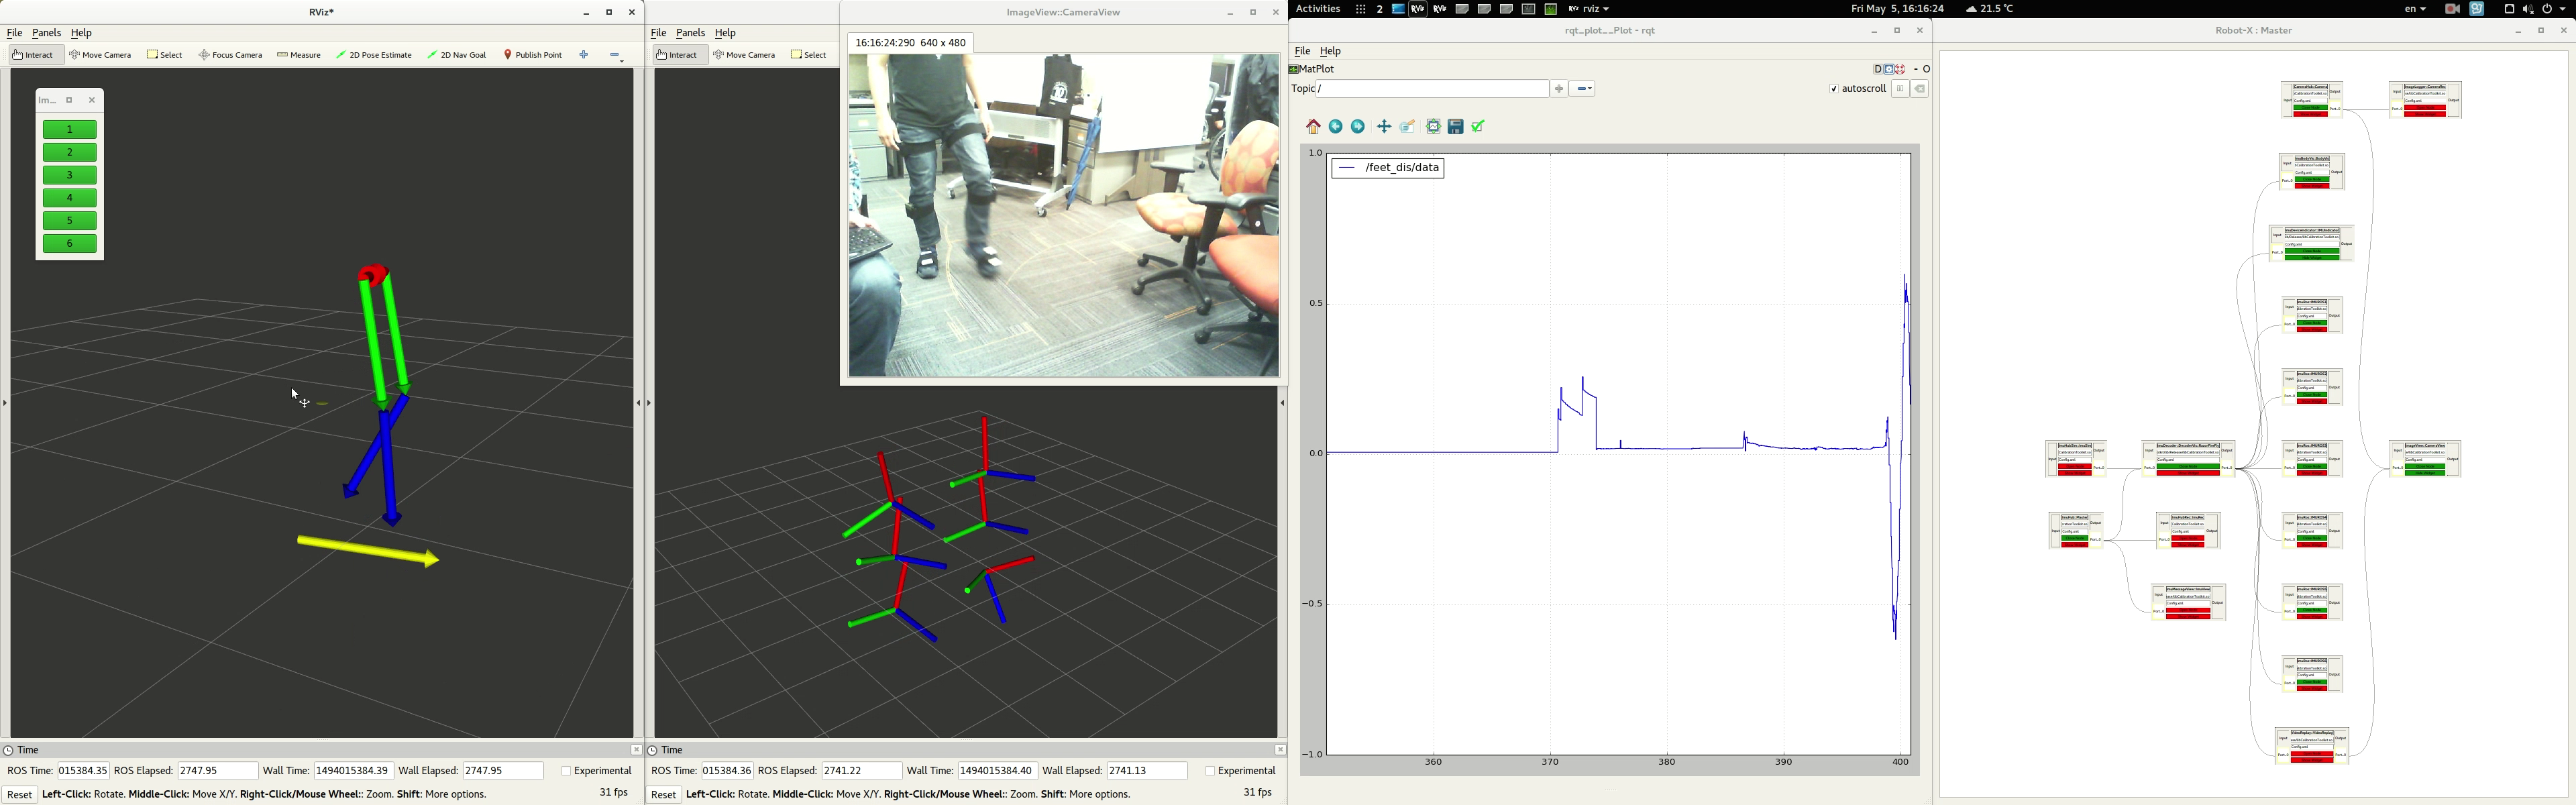
\includegraphics[width=0.95\columnwidth]{figs/vis}
  \caption{{\bf Final visualization layout}}
  \label{fig:vis }
\end{figure}

\subsection{Gait parameter graphs}
In adition to visualizing a subject's movements, our system can generate graphs of a
subject's knee extension and stride length in real time. Figure~\ref{fig:extend} shows the
graph of knee extension on the right as our subject bends his knee. The graph contains
separate extension angles for the left and right knee, so it is simple to notice if the
range of motion in one knee is more restricted than the other. 

\begin{figure}[h]
  \centering
  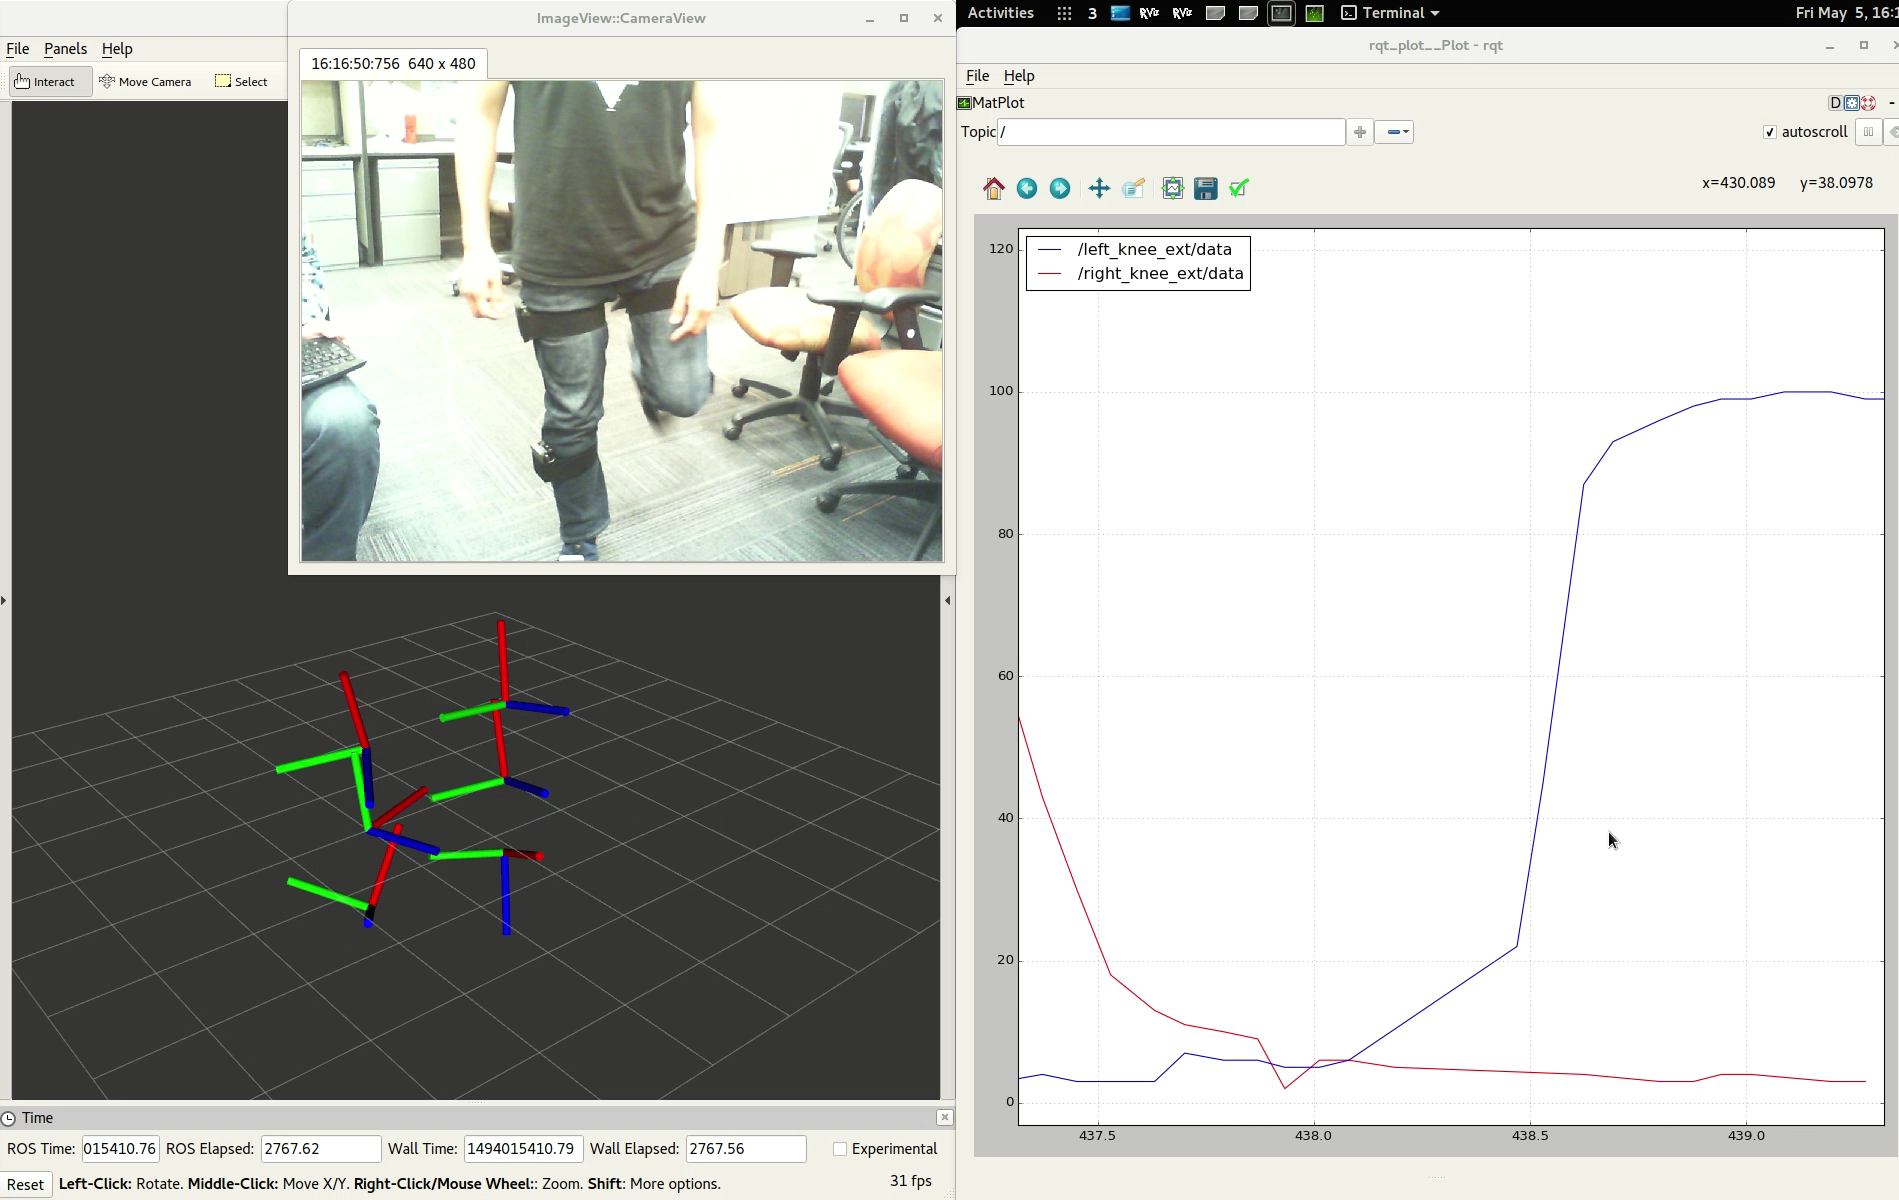
\includegraphics[width=0.95\columnwidth]{figs/extend}
  \caption{{\bf Real time knee extension reporting}}
  \label{fig:extend }
\end{figure}

The stride length graph appears in nearly real time, but requires additional processing
of the segments of multiple data points to find where steps occur, thus delaying it
slightly behind real time. However, it still provides useful, prompt feedback on the
length of a subject's stride as shown in Figure~\ref{fig:length}. The graph shows the
distance between the right and left foot, so the rise and fall pattern observed in the
graph in this figure indicates the feet separating as a subject's leg moves forward and coming
back together as the subject swings one foot past the other on the next step. 

\begin{figure}[h]
  \centering
  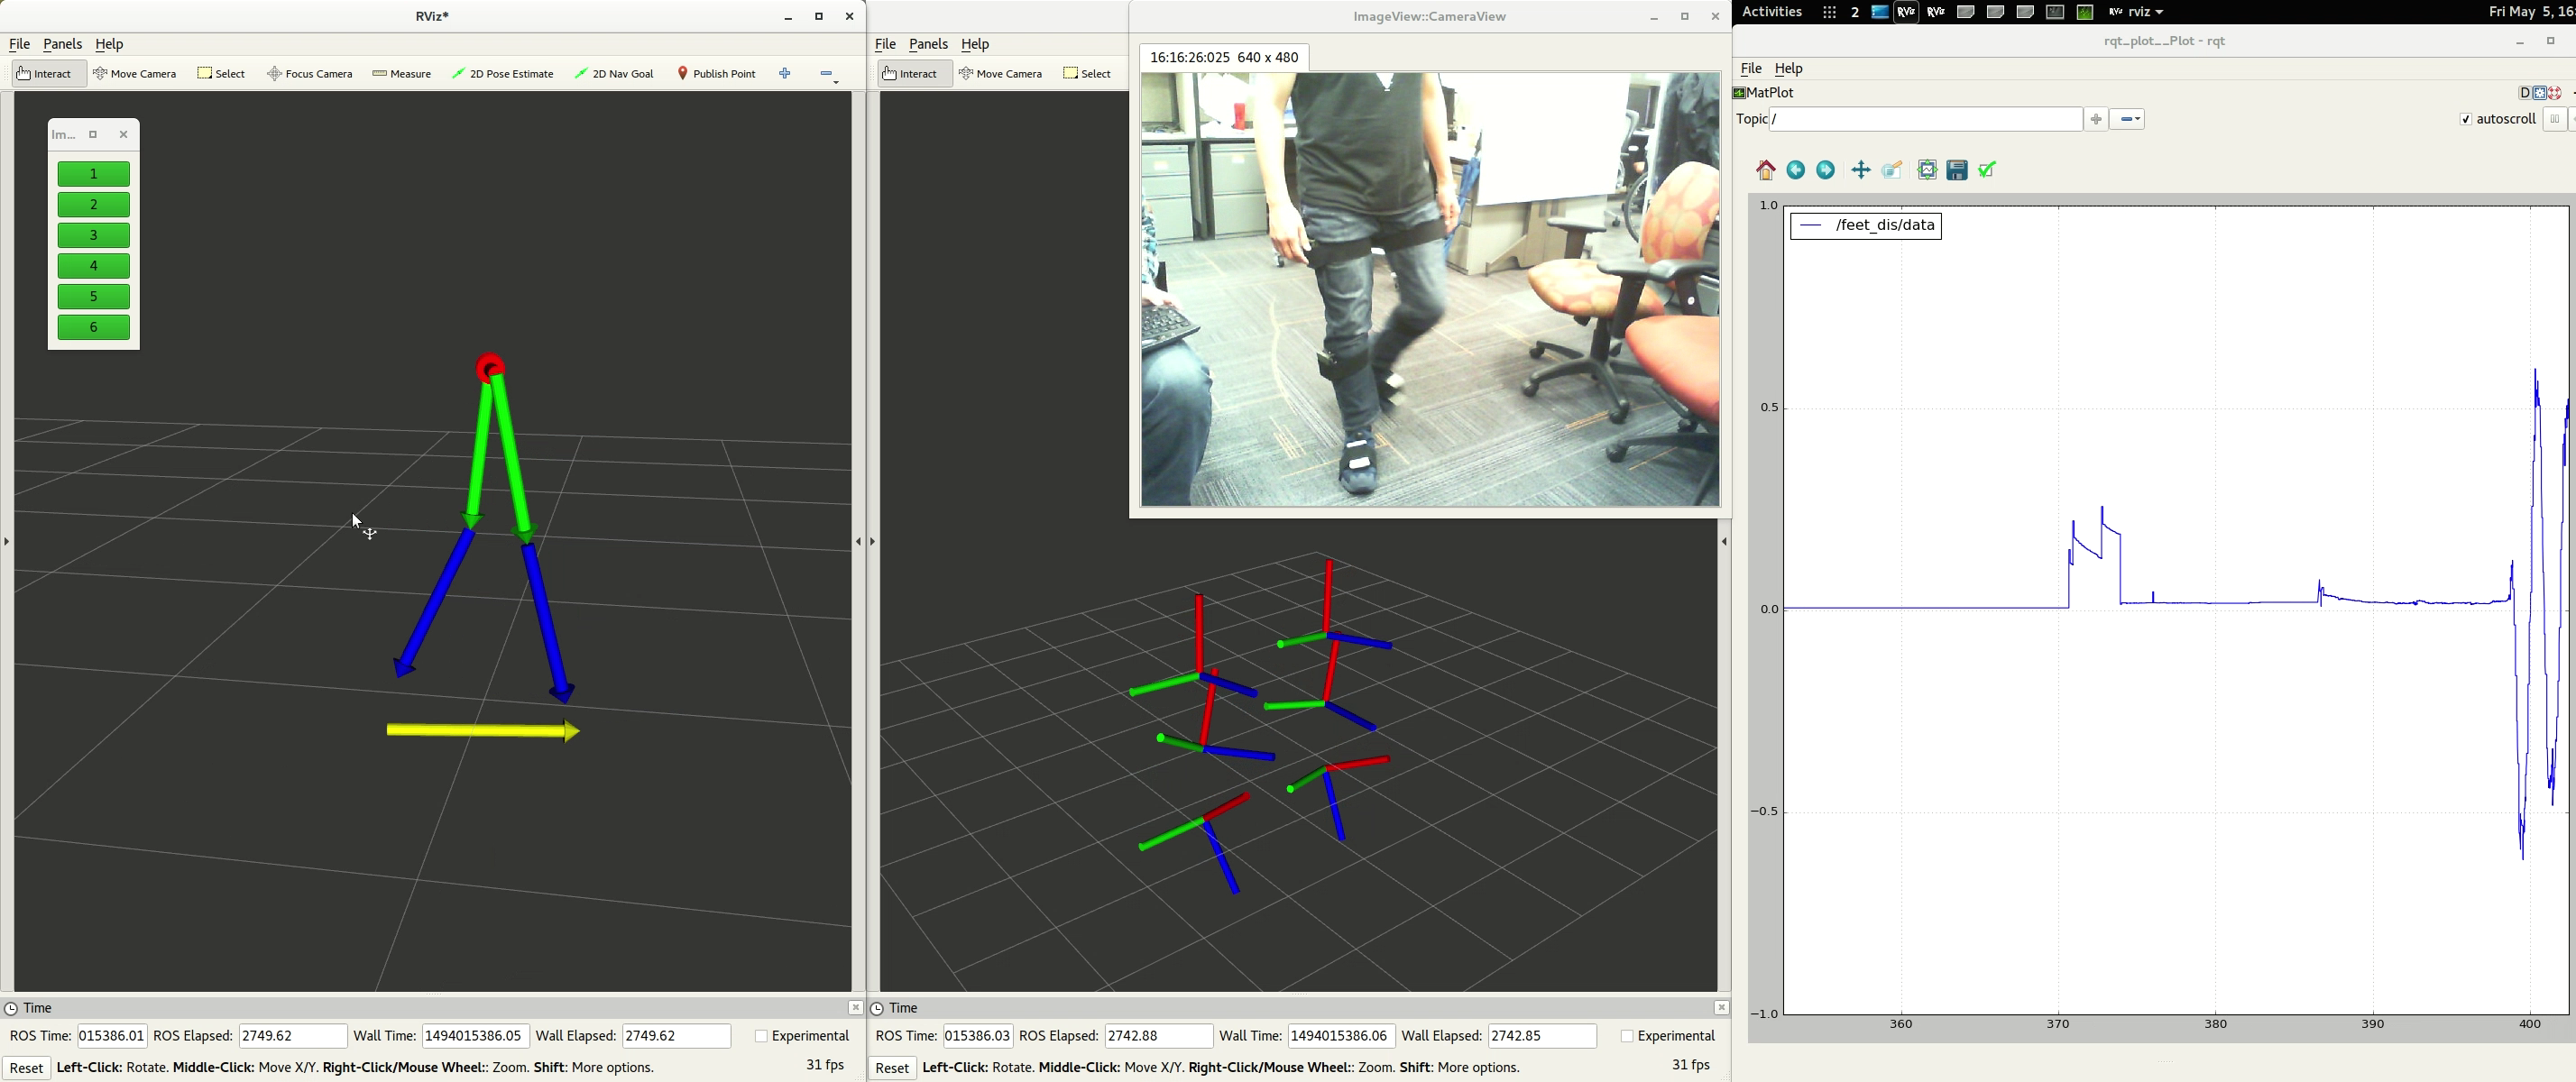
\includegraphics[width=0.95\columnwidth]{figs/length}
  \caption{{\bf Stride length reporting}}
  \label{fig:length}
\end{figure}

\subsection{Fall Detection}
In testing our gait monitoring system, we found that the orientation reported by the nodes
strapped to a patient's thighs provided a reliable fall indicator for our subject. When
the subject is walking, the measurement is stable and indicates that the node is
perpendicular to the ground plane. If a subject falls, the orientation data indicates a
rapid change in the angle between the node's central axis and the ground as demonstrated
in Figure~\ref{fig:falling}. Though our system relies primarily on the obvious change in
the grph that a system operator can visually observe, an automatic mechanism based on a
set threshold for the angle between the nodes and the ground would suffice to warn
caregivers that a patient has fallen. 

\begin{figure}[h]
  \centering
  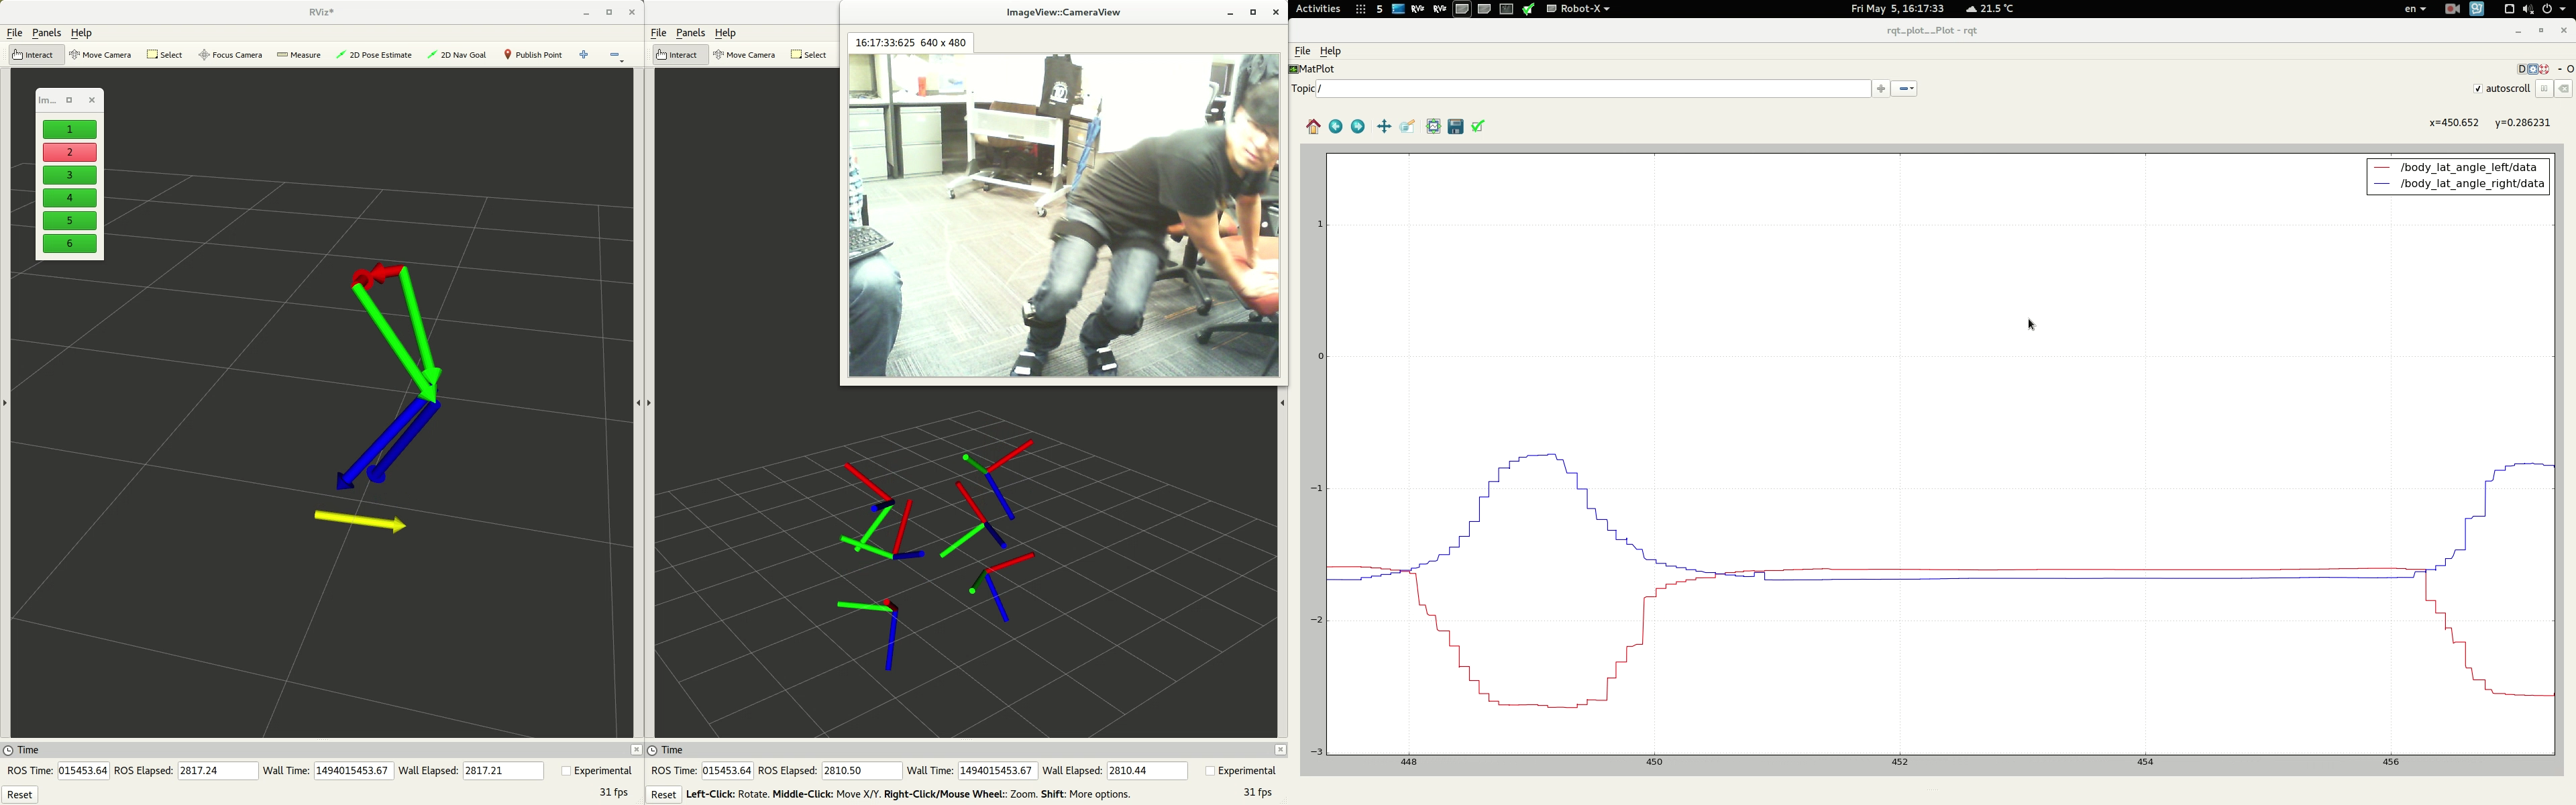
\includegraphics[width=.99\columnwidth]{figs/falling}
  \caption{{\bf Angle reporting for fall detection }}
  \label{fig:falling}
\end{figure}

\section{Conclusion}
\sys is a proof-of-concept implementation of gait monitoring using low cost IMUs and
a small number of wireless sensors. We were able to measure relevant parameters of our
subject's gaits and visualize the data in an accessible fashion despite the relatively low
data transfer rate in our network. \sys represents an example of a low cost monitoring
solution for patients with fall risks, and it could provide additional data for healthcare
providers seeking to customize a plan of care to a patient's behavior outside of the
office. We worked through several major challenges including timing mismatch between the
IMU and the Firefly, packet loss in the network, IMU drift, and signal processing
subtleties.
\section{Milestones and Task Division}
We achieved most of the milestones that we set out to accomplish in our original project
proposal, though some of the deadlines for the different milestones shifted.
Figure~\ref{fig:table} is a timeline of our original deliverable schedule and an explanation
of when each deliverable was finished or how it changed. 

\begin{figure}[h]
  \centering
  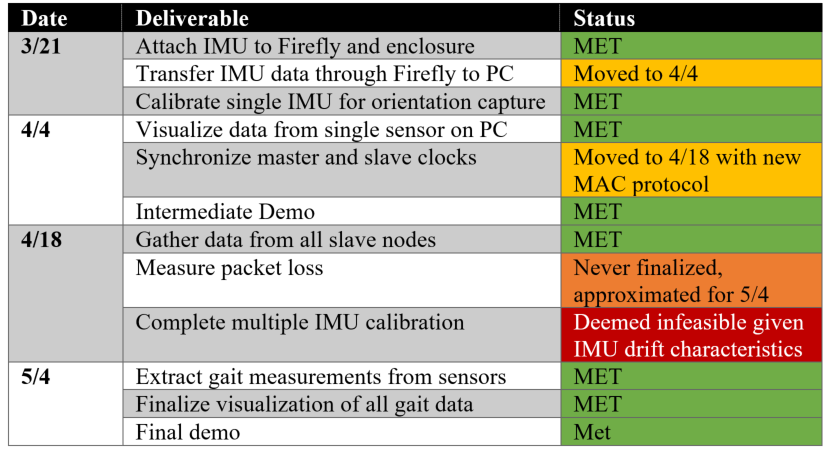
\includegraphics[width=\columnwidth]{figs/table}
  \caption{{\bf Timeline of deliverables }}
  \label{fig:table}
\end{figure}

The table below reports the segments of the project each team member completed.\\
\begin{tabular}{|p{.95\columnwidth}|}
  \hline
{\bf Alex:}
\begin{itemize}
  \item {IMU calibration feasibility assessment}
  \item ROS system development and management
  \item Motion capture and visualization
\end{itemize}\tabularnewline
\hline
{\bf Emily:}
\begin{itemize}
  \item{Data transfer from IMU to Firefly}
  \item{Inter-Firefly communication management}
  \item{Final report organization} 
\end{itemize}\tabularnewline
\hline
{\bf Iljoo:}
\begin{itemize}
  \item{Knee extension calculation} 
  \item{Step detection research and implementation}
  \item{Enclosure fabrication} 
\end{itemize}\tabularnewline
  \hline
\end{tabular}

\balance
\bibliographystyle{abbrv}
\bibliography{sigproc}  % sigproc.bib is the name of the Bibliography in this case
\end{document}

